\documentclass[a4paper,man,natbib]{apa6}

\usepackage[english]{babel}
\usepackage[utf8x]{inputenc}
\usepackage{amsmath}
\usepackage{graphicx}
\usepackage[colorinlistoftodos]{todonotes}

\usepackage{verbatim}
\usepackage{placeins}
\usepackage{float}
\usepackage{babel}
\restylefloat{figure}
\restylefloat{table}

\usepackage{tikz}
\usetikzlibrary{shapes,arrows}

% Modify Abstract title name from "Abstract" to "EXECUTIVE SUMMARY"
\addto{\captionsenglish}{\renewcommand{\abstractname}{EXECUTIVE SUMMARY}}

\title{\textbf{TROUBLESHOOTING AND DIAGNOSTIC ANALYSIS OF EARTH-MOVER SCRAPER --- CAT 637G}}
\shorttitle{CAT 637G --- Troubleshooting analysis }
\author{Prepared for

Lisa Slywka, Instructor

English and Communications

School of Applied Sciences and Technology
}
\affiliation{Prepared by

Tai Tran, 200222333

Industrial Heavy Equipment Technician Program

School of Applied Trades

October 31, 2016
}

%\abstract{}
    
\begin{document}

\centering The Northern Alberta Institute of Technology\\ Edmonton, Alberta

\maketitle

\tableofcontents
\newpage

\listoffigures
\newpage

\listoftables
\newpage



\section{INTRODUCTION}

% problem
``With today's highly sophisticated machinery and with the advent of mass production, industry can no longer afford a failure, as the cost of downtime is prohibitive.`` \citep[p. 190]{DodPracHyd}. To avoid these unexpected failures, techncians should recognize common symtoms and fix them before equipment breaks down.

\subsection{Purpose}

The goal of this report is to provide essential hydraulic and powertrain troubleshooting skills on Caterpillar scraper 637G. This research is significant due to the popularity of utilizing hydraulics in heavy equipment. As the vast majority of equipment heavily depends on hydraulics to do the job, including powertrain, technicians or students with troubleshooting skill in this field can consolidate their positions or increase the chances of getting a good job. In order to provide an in-depth analysis of the hydraulics and powertrain system, this report will not examine entire the 637G's hydraulic systems, which is not timely feasible.

\subsection{Background}

Just like a human body, if the owners and technicians neglect minor problems of equipment, things will get worse. Companies can have a comprehensive preventative maintenance strategy for their fleet; nevertheless, equipment still can fail at any time between service intervals because equipment health heavily relies on working environments. Hydraulic systems are very susceptible to contamination since components, such as cylinder seals are exposed to dusty environments. On the other hand, the powertrain might less prone to contamination as its components are less exposed. Therefore, their service life may be longer than other hydraulic systems, but their failures can cause longer downtime

%Understanding how to solve hydraulic and powertrain problems benefits both equipment owners and technicians. . 

\subsection{Scope}

Just like other heavy equipment, the 637G scraper uses hydraulics in many places: the bowl, apron, ejector, cushion-hitch, auger, steering, and powertrain. Because of the large amount of  hydraulic implementation used in the 637G, this paper will merely concentrate on the cushion-hitch, auger, and torque converter. Typically, the report will cover the purposes, locations, and basic diagnostic and troubleshooting knowledge for cushion-hitch, auger, and torque converter. Besides, the paper also incorporates safety procedures along with technical troubleshooting measures.

\section{EQUIPMENT DESCRIPTION}
\label{sec:examples}

\subsection{History Background}
 
Back in 1922, Robert Gilmour Letourneau and his brother-in-law Ray Peterson built the first earthmoving scraper in Stockton, California \citep[p. 35]{RLMBldng}. After the first scraper was built by Letourneau in 1922, the author created a second version of earthmoving scraper, nicknamed the Gondola. Later, the third edition Mountain Mover was created in 1923. The Self-Propelled scraper was the fourth built. Letourneau continuously dedicated his life to improve his creations \citep{RLMBldng}.

\begin{figure}[!ht]
\centering
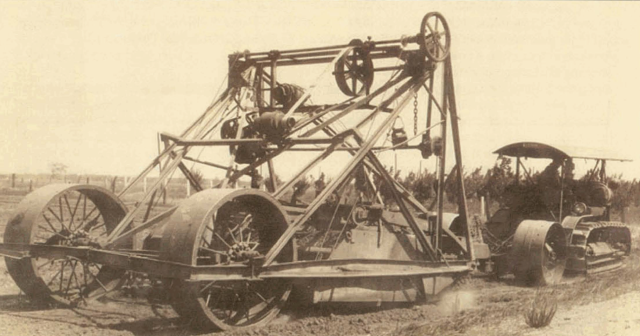
\includegraphics[width=0.5\textwidth]{mountain_mover_1922.png}
\centering\caption{\label{fig:rthcr1}Mountain Mover with a telescoping bowl was invented in June, 1922. \citep{RLMBldng}}
\end{figure}

\subsection{Components}

\section{Diagnostics and Troubleshooting Analysis}

\subsection{Hydraulic Systems}

\subsubsection{Cushion-hitch Hydraulic System}

\subsubsection{Auger Hydraulic System}

\subsection{Powertrain}

\subsubsection{Torque Converter}

\section{CONCLUSION}

\bibliography{main}

\end{document}


